% !TeX root = tlk16jun15h.tex
% !TeX encoding = UTF-8
% !TeX spellcheck = en_US


% !TeX encoding = UTF-8
% !TeX spellcheck = en_US

% !TeX root = ../m3Headout.tex
% !TeX encoding = UTF-8
% !TeX spellcheck = en_US

%% ==============================================================
%% ### BEAMER ###

\usetheme[]{CambridgeUS}	
\usecolortheme{seagull}			% seahorse, fly, dolphin, dove, beetle, seagull ...
\useinnertheme{circles}			% tree, smoothtree, infolines, smoothbars	
\usefonttheme{professionalfonts} 	% professionalfonts serif structurebold structureitalicserif structuresmallcapsserif
	
\beamertemplatenavigationsymbolsempty

%% ==============================================================
%% ### "PACKAGES" ###

% BY BEAMER: xcolor, amsmath, amsthm, calc, geometry, hyperref, extsizes

\usepackage{calc}

\usepackage[utf8x]{inputenc} 		% Eingabekodierung	
\usepackage[english]{babel}	
\usepackage[T1]{fontenc}	 		% Ausgabekodierung (PDF)
%\usepackage[
	%usenames,
	%dvipsnames,
	%svgnames,
	%table]{xcolor} 				% BEAMER, Farben
%\usepackage{amsmath}				% BEAMTER
%\usepackage{amsthm}				% BEAMTER
\usepackage{amssymb}				% \ngtpreq

\usepackage{proof} 					%\infer, \deduce
%\usepackage{marvosym}				% \Lightning

%\usepackage{soul}					% \so\caps\ul\st\hl
%\usepackage[normalem]{ulem} 		% \uline\uuline\sout\xout\uwave
%\usepackage{transparent}
\usepackage{listings} 			% are there some issues ?
%\usepackage{multirow}
%\usepackage{pdfpages}

%\usepackage[weather]{ifsym} 	% does not work with tex writer
%\let\Sun\relax 				% defined in marvosym too
%\let\Lightning\relax 			% defined in marvosym too

%\usepackage{ulsy}				% \blitza \blitzb ... \blitze (does not exist anymore? just not included?)

\usepackage{tabularx}

\usepackage{pifont} 			% dingbats

% setup listing

\lstdefinelanguage{smtlib}{
	comment={[l];},
	keywords={assert,xor, or, and},
	otherkeywords={declare-fun, set-logic},
	emph={Int,QF_LIA},
}

\lstset {
	backgroundcolor=\color{white},     	% choose the background color; you must add \usepackage{color} or \usepackage{xcolor}
	basicstyle=\ttfamily\footnotesize, 	% the size of the fonts that are used for the code
	breakatwhitespace=false,         	% sets if automatic breaks should only happen at whitespace
	breaklines=true,                 	% sets automatic line breaking
	captionpos=b,                    	% sets the caption-position to bottom
	commentstyle=\color{gray},    		% comment style
	deletekeywords={...},            	% if you want to delete keywords from the given language
	emphstyle=\color{orange},
	escapeinside={\%*}{*)},         % if you want to add LaTeX within your code
	extendedchars=true,             % lets you use non-ASCII characters; for 8-bits encodings only, does not work with UTF-8
	frame=none,		% frame=single, % adds a frame around the code
	keepspaces=true,                % keeps spaces in text, useful for keeping indentation of code (possibly needs columns=flexible)
	keywordstyle=\color{blue},      % keyword style
	% language=smtlib,	%Octave,    % the language of the code
	% literate={;},
	% otherkeywords={declare-fun,set-logic,assert,xor,or,and},            % if you want to add more keywords to the set
	%morecomment=[l]{;}				% line comment
	numbers=left,                   % where to put the line-numbers; possible values are (none, left, right)
	numbersep=5pt,                  % how far the line-numbers are from the code
	numberstyle=\tiny\color{gray}, 	% the style that is used for the line-numbers
	rulecolor=\color{black},        % if not set, the frame-color may be changed on line-breaks within not-black text (e.g. comments (green here))
	showspaces=false,               % show spaces everywhere adding particular underscores; it overrides 'showstringspaces'
	showstringspaces=false,         % underline spaces within strings only
	showtabs=false,                 % show tabs within strings adding particular underscores
	stepnumber=2,                   % the step between two line-numbers. If it's 1, each line will be numbered
	stringstyle=\color{orange},     % string literal style
	tabsize=2,	                   	% sets default tabsize to 2 spaces
	title=\lstname                  % show the filename of files included with \lstinputlisting; also try caption instead of title
}

% !TeX root = ../m3Handout.tex
% !TeX encoding = UTF-8
% !TeX spellcheck = en_US

%% color definitions

%\colorlet{col:a}{Fuchsia}
%\colorlet{col:b}{Blue}
\colorlet{colG}{Gray}
\colorlet{colO}{Orange}
\colorlet{colHi}{Green}
\colorlet{colLo}{Red}
\colorlet{colNa}{Gray}
\colorlet{colN}{Blue}
\colorlet{colEm}{RoyalBlue}
\colorlet{colMax}{Violet}
\colorlet{colSmx}{RoyalBlue}

%\newcommand{\colA}{\color{col:a}}	% example a
%\newcommand{\colB}{\color{col:b}}	% example b
\newcommand{\colG}{\color{colG}}	% neutral
%\newcommand{\colO}{\color{col:o}}	% old
\newcommand{\colN}{\color{colN}}	% new
\newcommand{\colHi}{\color{colHi}}	% hi, true
\newcommand{\colLo}{\color{colLo}}	% lo, false
\newcommand{\colNA}{\color{colNa}}	% not available		
\newcommand{\colMax}{\color{colMax}}	% maximal
\newcommand{\colSmx}{\color{colSmx}}	% strictly maximal		

%\newcommand{\MYa}{\color{Fuchsia}}
%\newcommand{\MYb}{\color{Blue}}
%\newcommand{\MYg}{\color{Gray}}
%\newcommand{\MYo}{\color{Orange}}
%
%\newcommand{\MYhi}{\color{Green}}
%\newcommand{\MYlo}{\color{Red}}
%\newcommand{\MYna}{\color{Gray}}
%
%\newcommand{\MYA}[1]{{\MYa#1}}
%\newcommand{\MYB}[1]{{\MYb#1}}
%\newcommand{\MYG}[1]{{\MYg#1}}
%\newcommand{\MYO}[1]{{\MYo#1}}
%
%\newcommand{\MYHI}[1]{{\MYhi#1}}
%\newcommand{\MYLO}[1]{{\MYlo#1}}
%\newcommand{\MYNA}[1]{{\MYna#1}}
%
%\newcommand{\MYS}[1]{{\color{Violet}#1}}
%\newcommand{\MYM}[1]{{\color{RoyalBlue}#1}}
%
%\newcommand{\mLightning}{{\text{\Lightning}}}

\newcommand{\BEGINX}{\begin{example}}
\newcommand{\ENDX}{\end{example}}

\newcommand{\BEGIN}{\begin{exampleblock}}
\newcommand{\END}{\end{exampleblock}}

\newcommand{\FOL}{$_\mathtt{FOL}$}
% !TeX root = ../m3Handout.tex
% !TeX encoding = UTF-8
% !TeX spellcheck = en_US

%% ==============================================================
%% ### MISC ###

%\newcommand{\EQ}{\simeq}
%\newcommand{\NEQ}{\not\simeq}
\newcommand{\foEQ}{\approx}		%	{\simeq}
\newcommand{\foNEQ}{\not\foEQ}

\newcommand\TOP[2]{\genfrac{}{}{0pt}{}{#1}{#2}}
\newcommand\TOPTEXT[2]{\TOP{\text{#1}}{\text{#2}}}
%\newcommand{\mygreek}[1]{\selectlanguage{polutonikogreek}#1\selectlanguage{english}}
%\newcommand{\mygreek}[1]{{\selectlanguage{polutonikogreek}#1}\selectlanguage{english}}
%\renewcommand{\mygreek}[1]{\foreignlanguage{polutonikogreek}{#1}}

%\newcommand{\iSUB}[2]{#2\!\mapsto\!#1}
%\newcommand{\BgSyntaxTree}{\usebackgroundtemplate{\transparent{0.1}\includegraphics[width=\paperwidth]{SyntaxTreeBackground.png}}}

\newcommand{\EMPH}[1]{\emph{\textcolor{colEm}{#1}}}

%% ==============================================================
%% ### MY MATH ENVIRONMENTS ###

\theoremstyle{plain}
%\newtheorem{theorem}{Theorem}
%\newtheorem{proposition}{Proposition}
%\newtheorem{lemma}{Lemma}
%\newtheorem*{corollary}{Corollary}

\theoremstyle{definition}
%\newtheorem{definition}{Definition}
\newtheorem{Conjecture}{Conjecture}
%\newtheorem*{example}{Example}
%\newtheorem{algorithm}{Algorithm}
\newtheorem{procedure}{Procedure}
\newtheorem{goal}{Goal}
\newtheorem{notation}{Notation}

\theoremstyle{remark}
%\newtheorem*{remark}{Remark}
\newtheorem*{observation}{Observation}
%\newtheorem*{note}{Note}
%\newtheorem{case}{Case}

%% ==============================================================
%% ### MY MATH DEFINITIONS ###

% math operators

%\DeclareMathOperator{\arity}{arity}
%\DeclareMathOperator{\var}{var}
%\DeclareMathOperator{\pos}{pos}
%\DeclareMathOperator{\T}{T}
%\DeclareMathOperator{\dom}{dom}
%\DeclareMathOperator{\rng}{rng}
%\DeclareMathOperator{\img}{img}
\DeclareMathOperator{\mgu}{mgu}	% most general unifier
%\DeclareMathOperator{\wgt}{W\!}
\DeclareMathOperator{\sel}{sel}
%\DeclareMathOperator{\mul}{mul}
%\DeclareMathOperator{\add}{add}

\DeclareMathOperator{\UNIF}{unifiable}
\DeclareMathOperator{\INST}{instance}
\DeclareMathOperator{\GNRL}{generalization}
\DeclareMathOperator{\VRNT}{variant}
\DeclareMathOperator{\PSTR}{pstr}

\newcommand{\NGTPREQ}{\not\succcurlyeq}

% constant (function, predicate) symbols

\newcommand{\mf}{{\mathsf f}}
\newcommand{\mg}{{\mathsf g}}
\newcommand{\mh}{{\mathsf h}}
\newcommand{\ma}{{\mathsf a}}
\newcommand{\mb}{{\mathsf b}}
\newcommand{\mc}{{\mathsf c}}
\newcommand{\md}{{\mathsf d}}
\newcommand{\mx}{{\mathsf x}}
\newcommand{\my}{{\mathsf y}}
\newcommand{\msucc}{{\mathsf s}}
\newcommand{\mpred}{{\mathsf p}}
\newcommand{\mA}{{\mathsf A}}
\newcommand{\mB}{{\mathsf B}}
\newcommand{\mL}{{\mathsf L}}
\newcommand{\mP}{{\mathsf P}}
\newcommand{\mQ}{{\mathsf Q}}

% caligraphic symbols

\newcommand{\mcC}{{\mathcal C}}
\newcommand{\mcD}{{\mathcal D}}
%\newcommand{\mcE}{{\mathcal E}}
%\newcommand{\mcF}{{\mathcal F}}
%\newcommand{\mcM}{{\mathcal M}}
%\newcommand{\mcO}{{\mathcal O}}
\newcommand{\mcP}{{\mathcal P}}
%\newcommand{\mcR}{{\mathcal R}}
%\newcommand{\mcT}{{\mathcal T}}
\newcommand{\mcV}{{\mathcal V}}

\newcommand{\Var}{{}\mcV\mathsf{ar}}
\newcommand{\Dom}{{}\mcD\mathsf{om}}
\newcommand{\Pos}{{}\mcP\mathsf{os}}
\newcommand{\PosStr}{\Pos^\Sigma}

% fraktal symbols

\newcommand{\mfC}{{\mathfrak C}}
\newcommand{\mfL}{{\mathfrak L}}
\newcommand{\mfR}{{\mathfrak R}}
\newcommand{\mfT}{{\mathfrak T}}

\newcommand{\SIGA}{{\mathcal A}}
\newcommand{\SIGC}{{\mathcal C}}
\newcommand{\SIGE}{{\mathcal E}}
\newcommand{\SIGF}{{\mathcal F}}
\newcommand{\SIGL}{{\mathcal L}}
\newcommand{\SIGP}{{\mathcal P}}
\newcommand{\SIGS}{{\mathcal S}}
\newcommand{\SIGT}{{\mathcal T}}
\newcommand{\SIGV}{{\mathcal V}}
% tt symbols

\newcommand{\mtS}{{\mathtt S}}
\newcommand{\sgr}{\succ_{\mathsf gr}}

% 

\newcommand{\TI}[1]{^{^{#1:}}\!}
\newcommand{\ANGLES}[1]{\langle#1\rangle}

\newcommand{\joins}{\rightarrow^*\cdot^*\!\!\leftarrow}
\newcommand{\meets}{^*\!\!\leftarrow \cdot \rightarrow^* }


\newcommand{\mCP}[1]{\mathsf{CP}(#1)}		% Critical Pair
\newcommand{\mCPR}{\mCP{\mcR}}		% CP(R)

\newcommand{\MUL}[2]	% multiplication
{\mf(#1,#2)}			% mul(x,y)
%{#1\cdot #2}			% x.y

\newcommand{\ADD}[2]	% addition
{\add(#1,#2)}			% add(x,y)
%{#1+#2}				% x+y

\newcommand{\MYPOS}[1]{{\tt #1}}
\newcommand{\overlap}[3]{\langle #1,\MYPOS{#2}, #3 \rangle}
\newcommand{\overlapN}[4]{{_{\overlap{#1}{#2}{#3}}}^{#4:\;}}

%\newcommand{\GTKBO}{>_{\tt kbo}}
\newcommand{\GTKBOW}[2]{\texttt{SMT}(#1\!>_\texttt{kbo}\!#2)}
\newcommand{\GTKBOP}[2]{\texttt{SMT}(#1\!>_\texttt{kbo}'\!#2)}

\newcommand{\UPL}{\infer
	[(\sigma)
		\quad\sigma=\mgu(l,l'), l'\!\not\in\mcV, l\sigma\rho\sgr r\sigma\rho
	]
	{L[r]\sigma}
	{l=r & L[l']}	
}

\newcommand{\emptyclause}{\square}

\newcommand{\cmark}{\ding{51}}
\newcommand{\xmark}{\ding{55}}

% !TeX root = ../m3Handout.tex
% !TeX encoding = UTF-8
% !TeX spellcheck = en_US

%% ### TIKZ ###

\usepackage{tikz}
\usetikzlibrary{
	automata,
	arrows,
	% backgrounds
	% decorations % --> pdflatex error
	% decorations.pathmorphing
	% fit,
	% graphs,p
	% petri,
	% positioning,
	% snakes -> decorations
	% shadows,
	shapes,
	trees,
}

\tikzset{
%	->,
%	>=stealth', 
%	shorten >=1pt, 
%	auto,
 	node distance=2.1cm, 
%	semithick,
 	minimum size=0,
 	inner sep=1,
 	outer sep=1mm,
%
 	initial text=$\varepsilon$,
%	
 	every state/.style={
 		fill=red,
%		draw=none,
%		text=white,
 		radius=0.1em
 	},
 	my/.style={ rectangle, draw=red	},
%	sloped,below
 }


\tikzstyle{myrect} = [rectangle,draw=black,rounded corners, minimum height=3em, thick, text centered,text width=5.5em]
\tikzstyle{mykaro} = [diamond,draw=black,rounded corners, thick, text centered,text width=4em]
\tikzstyle{mycircle} = [circle,draw=black,thick, text centered, minimum height=3.5em,text width=4em,text width=3.5em]
\tikzstyle{myarrow} = [thick,->,>=stealth]
%
\tikzstyle{myframe} = [rectangle,draw=black,rounded corners, minimum height=3em, thick, text centered,text width=5.5em]

%% ==============================================================

 \newcommand{\ORIGIN}{
 	\node[orange](ORIGIN) at (0,0) {\scriptsize$\odot$};
 	\node[orange](XONE) at (1,0) {\scriptsize$\times$};
 	}
%% ==============================================================

%copied from  m2report

 \tikzstyle{myrect} = [rectangle,draw=black,rounded corners, minimum height=3em, thick, text centered,text width=5.5em]
 \tikzstyle{mykaro} = [diamond,draw=black,rounded corners, thick, text centered,text width=4em]
 \tikzstyle{mycircle} = [circle,draw=black,thick, text centered, minimum height=3.5em,text width=4em,text width=3.5em]
 \tikzstyle{myarrow} = [thick,->,>=stealth]

 \tikzstyle{myframe} = [rectangle,draw=black,rounded corners, minimum height=3em, thick, text centered,text width=5.5em]

% clear command for final version

\renewcommand{\ORIGIN}{}
\providecommand{\PAUSE}{}






% ********************************

\author{Alexander Maringele}
\title{flea\\
}
%\subtitle{of an instantiation-based first order theorem prover with equality}
\subtitle{bit(e)s and pieces}
%\subtitle{in easy examples}
\date{June 15th, 2016}
%======

%\includeonly{DiscriminationTree}
\begin{document}

\selectlanguage{english}

\frame[<+->]{
\maketitle
} 

\frame{
	
	
	\begin{quote}
		Hofstadter's Law: It always takes longer than you expect, 
		
		even when you take into account Hofstadter's Law.
	\end{quote}
	 \hfill--- Douglas Hofstadter, Gödel, Escher, Bach: An Eternal Golden Braid
	}

\frame{
	\setcounter{tocdepth}{1}
	\tableofcontents}

%\include{Title}
\section*{References}
\frame[<+->]{
\frametitle{References}

\nocite{NHRV2001ote}
%\nocite{ SRV2001ti,ZHM2009jar,RV2003eir,NHRV2001ote}	% ZHM2009jar, RV2003eir, NHRV2001ote
\bibliographystyle{amsalpha}
\bibliography{biblio}

}
%\include{Overview}

%====================================================================
% BEGIN: CONTENT ----------------------------------------------------
%====================================================================

\section{Previously}

\subsection{First-order refutation}

\begin{frame}
	% We transform a first formula in to a equisatisfiable set of clauses,
	% i.e. the conjunction of universally quantified disjunction of variable distinct first order literals
	% then we check if the set is satisfiable, if not then the formula is a theorem.
	\frametitle{Goal}
	
	% !TeX spellcheck = en_US
% !TeX encoding = UTF-8

\begin{tikzpicture}[scale = 1, transform shape, draw=black, fill=black, thick, sloped]

	\draw[myarrow, ultra thick] (0,0) -- 
	node[pos=0, above] {$F$} 
	(2,0);
		
	% outer rectangle
	\draw[rounded corners=1.5mm,dotted] (0.5,3) rectangle (8.5,-3);
	% is F a theorem?
	\draw(1.9,2.7) node {Is $F$ a theorem?};
	
\pause
	% SLIDE Is S satisfiable?
	\node[colG] (S) at (1.1,-2.7) {\scriptsize$\lnot F \approx S$};
\pause
		\node (S) at (2.5,0) {$S$};
		

			% SLIDE 2
			\draw[thin,dashed,draw=colO] (2.5,0) ellipse (0.4 and 1.2); % S
			
			% inner rectangle
			\draw[very thick,draw=DarkGray]  (1.5,-2.25) rectangle (8,2.25); 
			% is S satisfaible?
			\draw (2.9,1.9) node {Is $S$ satisfiable?};
	
\pause
		% SLIDE unsatisfiable
		\draw[thin,dashed,draw=colO] (2.6,0) ellipse (0.6 and 1.44);  % S
		\draw[dashed, draw=colG, thick] 
		decorate[decoration={snake}] 
		{(1.4, 1) -- (8.2,0.6)};
		\draw[myarrow, draw=colHi, ultra thick] (6.5,1.8) -- 
			node[pos=0,below] {unsatisfiable}
			node[pos=0.85, above] {theorem} 
			(10,1.8) ;

\pause
		% SLIDE satisfiable
		\draw[thin,dashed,draw=colO] (2.8,0) ellipse (0.9 and 1.73);  % S
		\draw[dashed, draw=colG, thick]  
		decorate[decoration={snake}] 
		{ (1.4,-1)  --  (8.2,-0.6) };
		\draw[myarrow,draw=colLo, ultra thick] (7,-1.3) -- 
			node[pos=0, below] {satisfiable}
			node[pos=0.75, above] {not a theorem} (11,-1.3) ;
		 
\pause
		% SLIDE 5
		 \draw[thin,dashed,draw=colO] (3.2,0) ellipse (1.35 and 2.07); % S
		 	\draw[myarrow,draw=colNa, ultra thick] (7,0.15) -- 
		 	%	node[pos=0,above] {space out}
		 	node[pos=0,below] {time out}
		 	node[pos=0.85, above] {maybe} (10.5,0.15) ;

	\onslide<1->
\end{tikzpicture}
	
\end{frame}

\subsection{Resolution and InstGen}

\frame{
	\begin{Definition}[Ordered Resolution]
		% !TeX spellcheck = en_US
% !TeX encoding = UTF-8


\[
	\infer
	[]
	{(C \lor D)\sigma}
	{A \lor C& \lnot B\lor D}
%		\qquad
%		\infer[]
%		{C\sigma}
%		{A\lor\lnot B\lor C}
		\]
		where 
		\begin{center}
		$A\sigma$ strictly maximal in $\mcC\sigma$, $\lnot B\sigma$ maximal in $\mcD\sigma$, $\sigma=\mgu(A,B)$.
		\end{center}
		\end{Definition}
	
	\begin{Definition}[Inst-Gen]
	% !TeX spellcheck = en_US
% !TeX encoding = UTF-8


\[
	\infer
	[]
	{(A \lor \mcC)\sigma\quad(\lnot B\lor \mcD)\sigma}
	{A \lor \mcC& \lnot \mc\lor D}
	\]
	where
	\[
		\sel(A\lor\mcC) = A\qquad\sel(\lnot B\lor \mcD) = \lnot{B}\qquad\sigma=\mgu(A,B)
	\]
\end{Definition}

%\begin{Example}[Unsatisfiable set of clauses]
%	$S = \{ \mP(x)\lor\lnot\mP(y), \lnot\mP(\ma),\mP(\mb)\}$
%\end{Example}
}

\subsection{Examples}
\frame{
	\begin{Example}[Resolution]
		\vspace{-1em}
		% !TeX root = tlk16jun15h.tex

	\vspace{-1.5em}
\begin{gather*}
	S = 
	\{ 
	\mP(x) \lor \lnot\mP(y), 
	\lnot \mP(\ma), 
	\mP(\mb) 
	\}\\[0.5em]
\infer[y\mapsto\mb]{\emptyclause}{
\infer[x\mapsto\ma]{\lnot\mP(y)}{\mP(x)\lor \lnot \mP(y) & \lnot\mP(\ma)} & \mP(\mb)
	}
			\end{gather*}
		\end{Example}
		
			\begin{Example}[Inst-Gen]
				\vspace{-1em}
				\begin{align*}
	S_0\bot =&\  
	\{ 
	{\colHi\mP(\bot)} \lor \lnot\mP(\bot), 
	{\colHi\lnot \mP(\ma)}, 
	{\colHi\mP(\mb)} 
		\} \tag{satisfiable} \\
		&\quad 
		\infer[x\mapsto\ma]{
			\mP(\ma)\lor\lnot\mP(y)
			}{\mP(x)\lor\lnot\mP(y))&\lnot\mP(\ma)}
			\\
			S_1\bot \supsetneq&\  
			\{  
			{\colHi\lnot \mP(\ma)}, 
			{\colHi\mP(\mb)},
				{\colLo\mP(\ma)} \lor {\colHi \lnot \mP(\bot) } \}
				\tag{satisfiable}
				\\
				&\quad
				\infer[y\mapsto\mb]{
					\mP(\ma)\lor\mP(\mb)}{
					\mP(\mb)&\mP(\ma)\lor\lnot\mP(y)
					}
					\\
					S_2\bot \supsetneq&\ 
					\{ \lnot\mP(\ma), \mP(\mb), \mP(\ma) \lor \lnot\mP(\mb) \} \tag{unsatisfiable}
	\end{align*}
			\end{Example}
		}
		
	

		



\section{Procedure}

% !TeX root = tlk16jun15h.tex


\subsection{Run-Loop}

\frame{\begin{block}{Run-Loop}
%\begin{figure}[hbt]
\begin{center}
\begin{tikzpicture}[scale=0.75, transform shape]
\node[rectangle] (start) at (0,-4em) {};
\node (nc) [myrect] at (0,0) {new\\clauses};
\node (pc) [myrect] at (0,8em) {passive clauses};
\node (ab) [myrect] at (-8em,3.5em) {instantiation};
\node (gs) [myrect] at (-8em,8em) {SMT};
\node (un) [mycircle,colHi,very thick] at (-15em,8em) {un\-satis\-fiable};
\node (se) [myrect] at (-8em,12.5em) {selection};
\node (gc) [myrect] at (0em,16em) {given clause};
\node (ac) [myrect,dashed] at (-14em,16.5em) {active clauses};

\node (sl) [myrect, thick] at (8em,12.5em) {selected literal};
\node (us) [myrect] at (8em,8em) {search for conflicts};
\node (sa) [mycircle, very thick,colLo] at (15em,8em) {satis\-fiable};
\node (su) [myrect] at (8em,3.5em) {substitution};

\node (parse) [myrect,dotted]  at (14em,-2em) {read\\file(s)};

\draw[myarrow, dotted] (parse) to [bend left=20] (nc);
\draw[myarrow] (nc) to (pc);
\draw[myarrow] (nc.west)  to [bend left=10] (ab);
\draw[myarrow] (ab) to (gs);
\draw[myarrow] (gs) to (un);
\draw[myarrow] (gs) to (se);
\draw[myarrow] (pc) to (gc);
\draw[myarrow] (se.north) to [bend left=10] (gc.west);
\draw[myarrow] (us) to (sa);
\draw[myarrow] (us) to (su);
\draw[myarrow] (su) to [bend left=10] (nc.east);
\draw[myarrow] (sl) to (us);
\draw[myarrow] (gc.east) to [bend left=10] (sl.north);
%\draw[myarrow,dashed] (gc.north) to [bend right=15](ac);
\draw[myarrow, dashed] (gc) to [bend right=20] (ac);

\path (nc) edge [myarrow,loop below, dashed] (nc)
 (parse) edge [myarrow, loop above, dotted] (parse)
 (19em,-2em) edge [myarrow,dotted](parse)
;
\end{tikzpicture}
%\caption{Inst-Gen loop with maximal completion}
%\label{fig:inst-gen-maxcomp}
\end{center}
%\end{figure}
\end{block}}

\subsection{Redundancy}
		\frame{
			\begin{block}{Subsumption}
				\vspace{-1em}
%				Subsumed clauses can be removed from a set of first order clauses without affecting satisfiability.
%				Proper instances of clauses affect the satisfiability of the set of ground instances.
				\begin{gather*}
					S = \{C, D, \ldots \}\qquad \exists\theta\ C\theta\subseteq D 
					\tag*{C subsumes D}\\
					 S \text{ satisfiable} 
					 \overset{\text{\colHi\cmark}}\iff (S \setminus D) \text{ satisfiable }
%					   \tag*{Resolution}
					   \\
					   \theta\text{ is proper, }
					S\bot \text{ satisfiable}\ 
%					{\colLo\overset{\text{\colLo\xmark}}{\colLo\Leftarrow \Rightarrow}}
					{\colLo\overset{\text{\xmark}}{\Leftarrow\Rightarrow}}\
					(S \setminus D)\bot \text{ satisfiable } 
%					\tag*{Inst-Gen}
					\\
					\theta\text{ is renaming, }
					S\bot \text{ satisfiable} 
					{\overset{\text{\colHi\cmark}}\iff}
					(S \setminus D)\bot \text{ satisfiable } 
					\end{gather*}
				\end{block}
			
			\begin{Example}[]
				\vspace{-1em}
					\begin{gather*}
\{ 	\mP(x,y), \lnot\mP(\ma,z) \} 
\qquad 
\{ 	\mP(x,y), \lnot\mP(\ma,z), {\colG\mP(\ma,z)} \} 
\\
	\{ \mP(\bot,\bot), \lnot\mP(\ma,\bot) \} 
	\qquad 
	\{ \mP(\bot,\bot), {\lnot\mP(\ma,\bot)},{\colLo\mP(\ma,\bot)} \}
					\end{gather*}
				
				\end{Example}
%							\begin{block}{}
%								Proper instances of clauses affect the satisfiability of the set of ground instances.
%							\end{block}
			}
			
			\subsection{Data structures}
			\frame{
				\begin{block}{necessary data structures}
					\begin{enumerate}
						\item representation of clauses, literals and terms
						\item fast retrieval of clauses with a selected literal that is unifiable with the negation selected literal of a given clause
						\item fast retrieval of clauses with a set of literals that is a renamed subset of a given clause
					\end{enumerate}
					
					\end{block}
				}
				
				\subsection{Path indexing}
				\frame{
					% !TeX root = tlk16jun15h.tex
% !TeX encoding = UTF-8
% !TeX spellcheck = en_US

\begin{gather*}
	\{
	\TI{1}\mP(\mf(x,x)),
	\TI{2}\mP(\mg(\ma,x)), 
	\TI{3}\mP(\mf(y,z)),
	\TI{4}\mP(\mg(\ma,y)), 
	\TI{5}\mP(\mf(y,x)), 
	\TI{6}\mP(\mg(y,a))
	\}
\end{gather*}
%
\begin{center}
	\begin{tikzpicture}[->,sloped,above]
	
	\node (root) at (0,2.5) {.};
	
	\node (h) at (1,2.5) {.};
	
	\node (h1) at (2,2.5) {.};
	
	\node (h1f) at (3,4.5) {.};
	\node (h1g) at (3,1.5) {.};
	
	\node (h1f1) at (4,5) {.};
	\node (h1f2) at (4,4) {.};
	\node (h1g1) at (4,2.5) {.};
	\node (h1g2) at (4,0.5) {.};
	
	\node (h1f1x) at (6,5) {\{1,3,5\}};
	\node (h1f2x) at (6,4) {\{1,3,5\}};
	\node (h1g1a) at (6,3) {\{2,4\}};
	\node (h1g1x) at (6,2) {\{6\}};
	\node (h1g2a) at (6,1) {\{6\}};
	\node (h1g2x) at (6,0) {\{2,4\}};
	
	\path (root) edge node {$\mP$} (h)
	(h) edge node {$1$} (h1)
	
	(h1)
	edge node {$\mf$} (h1f)
	edge node {$\mg$} (h1g)
	
	(h1f)
	edge node {$1$} (h1f1)
	edge node {$2$} (h1f2)
	
	(h1g)
	edge node {$1$} (h1g1)
	edge node {$2$} (h1g2)
	
	(h1f1)
	% edge node {$\ma$} (h1f1a)
	edge node {$*$} (h1f1x)
	
	(h1f2)
	%		edge node {$\ma$} (h1f2a)
	edge node {$*$} (h1f2x)
	
	
	(h1g1)
	edge node {$\ma$} (h1g1a)
	edge node {$*$} (h1g1x)
	
	(h1g2) 
	edge node {$\ma$} (h1g2a)
	edge node {$*$} (h1g2x)
	
	(root)
	edge node {$\lnot$} (1,4)
	edge node {$\mQ$} (1,1)
	;
	\end{tikzpicture}
\end{center}
$\lnot\mP(\mg(\mb,z)) \mapsto \{ \mP.1.\mg.1.{\mb}, \mP.1.\mg.2.{*} \} \mapsto \{6\} \cap \{2,4,6\}$}
				
				\subsection{Discrimination trees}
				\frame{
					% !TeX root = ../m3Handout.tex
% !TeX encoding = UTF-8
% !TeX spellcheck = en_US

\begin{block}{Insert}
	\def\TRIEWIDTH{4cm}
	\def\TEXTWIDTH{\textwidth-\TRIEWIDTH-2em}
	\begin{minipage}{\TEXTWIDTH}
		$
\TI{\ell_1}\mP(\mf(x,y)), 
\TI{\ell_2}\mP(\mf(x,\mh(\ma))),
\TI{\ell_3}\mP(\mf(\mh(\ma),\ma))
$
		\begin{align*}
			t_1 &\Rightarrow \mh.\mf.{*}.{*}\\
			t_2 &\Rightarrow \mh.\mf.{*}.\mh.\ma \\
			t_3 &\Rightarrow \mh.\mf.\mh.\ma.\ma
			\end{align*}
	\end{minipage}
	\begin{minipage}{\TRIEWIDTH}
		\def\pyL{-0.3}
		\def\pxL{-0.0}
		\begin{tikzpicture}[->,dotted]
		\renewcommand{\PAUSE}{\pause}
		\ORIGIN

\def\pyL{-0.2}
\def\pxL{0.05}

\PAUSE

\node (root) at (2.5,5) {.};
\node (h) at (2.5,4) {.};
\path (root) edge node {$\mh$} (h);

\PAUSE
\node (h1) at (2.5,3) {.};
\path (h) edge node {$1$} (h1);

\PAUSE
\node (h1f) at (1.5,2) {.};
\path (h1) edge node {$\mf$} (h1f);

\PAUSE
\node (h1f1) at (0.5,1) {.};
\path (h1f) edge node {$1$} (h1f1);

\PAUSE
\node (h1f1x) at (0,0) {.};
\path (h1f1) edge node {$*$} (h1f1x);
\node (12) at (\pxL,\pyL) {\scriptsize$t_1,t_2$};

\PAUSE
\node (h1f1a) at (1,0) {.};
\path (h1f1) edge node {$\ma$} (h1f1a);
\node (3) at (\pxL+1,\pyL) {\scriptsize$t_3$};

\PAUSE
\node (h1f2) at (2.5,1) {.};
\path (h1f) edge node {$2$} (h1f2);

\PAUSE
\node (h1f2x) at (2,0) {.};
\path (h1f2) edge node {$*$} (h1f2x);
\node (1) at (\pxL+2,\pyL) {\scriptsize$t_1$};

\PAUSE
\node (h1f2a) at (3,0) {.};
\path (h1f2) edge node {$\ma$} (h1f2a);
\node (23) at (\pxL+3,\pyL) {\scriptsize$t_2,t_3$};


\node (lu) at (0,-0.5) {} ;
		\node (lu) at (-3,-5.5) {} ;
		\end{tikzpicture}
	\end{minipage}
	%
\end{block}
					
					\begin{block}{Implementation}
						\vspace{-1em}
%						The literal index is implemented as mapping from yices literals to clauses.
						
						\begin{align*}
							\texttt{ Clause}&\mapsto\mathtt{(Int,\ Set\ of\ term\_t)}\\
						\texttt{ term\_t}&\mapsto \mathtt{Set\ of\ Int}\\
							\texttt{ Int}&\mapsto \mathtt{Clause}
						\end{align*}
						
						\end{block}
					}
					
\subsection{Yices API}
\begin{frame}
\scalebox{0.8}[1.0]{\begin{minipage}{40em}
\texttt{{\colEm type\_t} yices\_bool\_type({\colEm void});}
\\[0.25em]							
\texttt{{\colEm type\_t} yices\_new\_uninterpreted\_type({\colEm void});}
\\[0.25em]							
\texttt{{\colEm type\_t} yices\_function\_type({\colEm uint32\_t} n, const {\colEm type\_t} dom{\colEm []}, {\colEm type\_t} range);}
\\[0.75em]							
\texttt{{\colEm term\_t} yices\_new\_uninterpreted\_term({\colEm type\_t} tau);}
\\[0.25em]
\texttt{{\colEm term\_t} yices\_application({\colEm term\_t} fun, {\colEm uint32\_t} n, const {\colEm term\_t} arg[]);}
\\[0.25em]
\texttt{{\colEm term\_t} yices\_eq({\colEm term\_t} left, {\colEm term\_t} right);}
\\[0.75em]
\texttt{{\colEm term\_t} yices\_not({\colEm term\_t} arg);}
\\[0.25em]
\texttt{{\colEm term\_t} yices\_or({\colEm uint32\_t} n, {\colEm term\_t} arg{\colEm []});}
\\[0.75em]
\texttt{{\colEm int32\_t} yices\_assert\_formula({\colEm context\_t *ctx}, {\colEm term\_t} t);}
\\[0.75em]
\texttt{{\colEm smt\_status\_t} yices\_check\_context({\colEm context\_t *}ctx, const {\colEm param\_t *}params);}
\\[0.25em]
\texttt{{\colEm model\_t} *yices\_get\_model({\colEm context\_t *}ctx, {\colEm int32\_t} keep\_subst);}
\\[0.25em]
\texttt{{\colEm int32\_t} yices\_get\_bool\_value({\colEm model\_t *}mdl, {\colEm term\_t} t, {\colEm int32\_t *}val);}

\end{minipage}}
							
							
						
	
						\end{frame}

\section{Equality}
\subsection{Schemata}

\begin{frame}
	\begin{block}{Schemata}
		\vspace{-1em}
		\begin{align*}		
			&x=x &s\neq s
			\\
			{\colG x\neq y\ \lor}\ 
				&y=x &s \neq t
			\\
			{\colG x\neq y \lor y\neq z\ \lor}\ 
				&x=z &s\neq t
			\\
			{\colG x_1\neq y_1 \lor x_2\neq y_2 \ \lor}\ 
			&\mf(x_1,x_2) = \mf(y_1,y_2) 
				&\mf(s)\neq\mf(t)
			\\
		    {\colG x\neq y\ \lor}\ &\lnot\mP(x) \lor \mP(y) 
			    &\mP(s), \lnot\mP(t)
			\end{align*}
		\end{block}
%		
		\begin{example}
			\vspace{-1em}
			\begin{align*}
			S =&\ \{ \mP(\ma), \lnot\mP(\mf(\ma,\mb)), \mf(x,\mb)= x \} 
			\\[0.5em]
%			&\quad\infer[
%			]{
%				\ma\neq y \lor \lnot \mP(\ma) \lor \mP(y)
%				}{
%				x\neq y \lor \lnot\mP(x) \lor \mP(y)  & \mP(\ma)
%			}
%				\\[0.5em]
%				&\quad\infer[
%				]{
%					x\neq \mf(\ma,\mb) \lor \lnot \mP(x) \lor \mP(\mf(\ma,\mb))
%				}{
%				x\neq y \lor \lnot\mP(x) \lor \mP(y) & \lnot\mP(\mf(\ma,\mb))
%			}
&\quad \ma\neq y \lor \lnot \mP(\ma) \lor \mP(y) \tag*{congruence}\\
&\quad x\neq \mf(\ma,\mb) \lor \lnot \mP(x) \lor \mP(\mf(\ma,\mb)) \tag*{congruence}
\end{align*}
			\end{example}
			
			\end{frame}


\section{Bernays–Schönfinkel-Ramsey}

\subsection{Effectively Propositional}

\begin{frame}
		
		
		
		\begin{block}{}
			The Bernays–Schönfinkel-Ramsey class of first-order formulae is a decidable fragment of first-order logic.
			%		 and can be effectively translated into propositional logic (EPR).
			Each formula in this fragment is equivalent to a satisfiable formula
			\[\exists a_1\ldots a_m \forall y_1\ldots\ y_n\,F\] 
			where $F$ is quantifier free and does not contain function symbols.
			
			
		\end{block}
		
		\begin{example}
			\vspace{-1em}
			\begin{gather*}
				\ma\neq x\lor\mQ(\ma,x), \mQ(y,\mb)
			\end{gather*}
		\end{example}
		
		\begin{block}{Remark}
			In practice the additon of equality axioms reduces the success rates of (instantiation-based) automated theorem provers drastically.
			\end{block}
		
	\end{frame}

\section{Summary and Outlook}



\frame{
	\begin{itemize}
		\item Done:
	\begin{itemize}
		\item Scanning and parsing with \texttt{flex} and \texttt{bison}
		\item Application logic with two simple strategies
		\item SMT Checking with Yices 2
	\end{itemize}
	\item Ongoing:
	\begin{itemize}
		\item Integration of Unit Superposition calculus
		\item Integration of Z3 for unsatisfiable core and maximal completion
		\item Tests and experiments
	\end{itemize}
	\item Missing:
	\begin{itemize}
		\item Good strategies
		\item Combinations of strategies
		\item Migration to Linux
	\end{itemize}
	\end{itemize}
	}
\subsection{optimization}

\frame{
	\begin{center}
	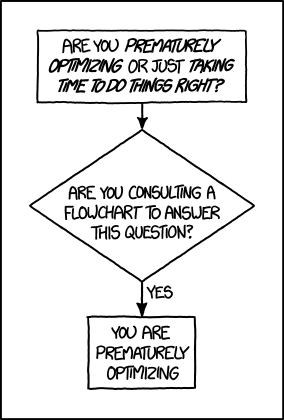
\includegraphics[scale=0.5]{../xkcd/optimization}
	\end{center}
	}
 
\end{document}